
\section{Experiments \& Analysis}
In this section, we first evaluate the performance of various models on M-DocSum-Bench using the inference prompt which can be found in the Appendix Figure~\ref{fig:prompt_infer} and compare M-DocSum-7B with several baselines. 
Then, we conduct an ablation study to analyze our key training steps and data.


\subsection{Main Results}
As shown in Table~\ref{tab:main}, M-DocSum-7B outperforms all open-source models in both text and image overall evaluations. 
Notably, in image referencing, M-DocSum-7B even surpasses advanced closed-source models, with its Image Score exceeding Gemini-Pro by 24\% and GPT-4o by 9\%. 
It is also the only model where both Overall Matching and Jaccard Similarity scores exceed 60\%, highlighting its proficiency in image understanding and referencing.
Some notable results include the exceptional performance in text generation completeness and accuracy for Gemini Pro.

Open-source models show that overall scores increase with model parameter size, with the Qwen2.5 series outperforming the Qwen2 series. 
For InternVL, the results indicate that the model is better at generating high-quality text but neglects the understanding and referencing of the images. 
Its None Accuracy score is nearly 1, suggesting that almost all predictions are ``None" which means that no images are selected.



\subsection{Analysis}

\subsubsection{Paragraph-wise Performance Variations}
Figure~\ref{fig:analysis}(a) reveals that models more accurately reference images in earlier paragraphs, with accuracy declining in later sections.
This might be because earlier images are more directly related to the text, while later images could involve more complexity. 
Figure~\ref{fig:analysis}(b) indicates that the task difficulty is well-calibrated with an average score around 0.55, showing distinct difficulty levels across paragraphs. 
Paragraph 4 scores the highest, reflecting strong summarization capabilities, likely due to its structured and key information-rich nature.
Paragraph 2 follows, indicating robust understanding and summarization of specific methods.
Paragraphs 1 and 3 (Background and Experimental Design) score lower, possibly because of their extensive detail and background information, challenging models in extraction and summarization.
The consistent trend observed across all models indicates that our paragraph and difficulty settings are reasonable and our evaluation is stable, leading to highly consistent results.
Detailed results can be found in the Appendix Section~\ref{Paragraph-wise Performance Variations}.

\subsubsection{Influence of Context Length on Performance}
Figures~\ref{fig:analysis}(c) and (d) illustrate a clear trend: as the context length increases, both text and image scores decrease. Notably, the decline in image scores is more precipitous than that of text scores. This disparity suggests that longer contexts disproportionately challenge the models' ability to accurately reference and integrate relevant images, likely stemming from the increased difficulty of localizing the correct visual information within extensive, multi-page documents. Furthermore, a performance gap is observed between open-source and closed-source models. Open-source models exhibit a steeper performance degradation with increasing context length, while closed-source models demonstrate greater robustness. This difference likely reflects the advantages of closed-source models in terms of larger-scale, higher-quality training data, and potentially more sophisticated training methodologies.
Detailed results can be found in the Appendix Section~\ref{Influence of Context Length on Performance}.

\subsubsection{Impact of Image Quantity on Performance}
Figure~\ref{fig:analysis}(e) reveals a significant decrease in image referencing scores across all models as the number of images per document increases. This highlights the challenge models face in selecting pertinent images for summarization in image-rich contexts. The highest scores are observed with documents containing only 1-3 images, suggesting that correct image selection is facilitated in these less visually complex scenarios.
Figure~\ref{fig:analysis}(f) illustrates that leading closed-source models sustain stable text scores irrespective of the image count. This consistency in text generation likely reflects their advanced architectural designs and optimization strategies. Conversely, open-source models, along with certain closed-source models, show a deterioration in text quality as the number of images grows, suggesting limitations in their multimodal integration capabilities, potentially attributable to constraints in model size and training data.
Detailed results can be found in the Appendix Section~\ref{Impact of Image Quantity on Performance}.


\begin{figure*}[t]
\centering
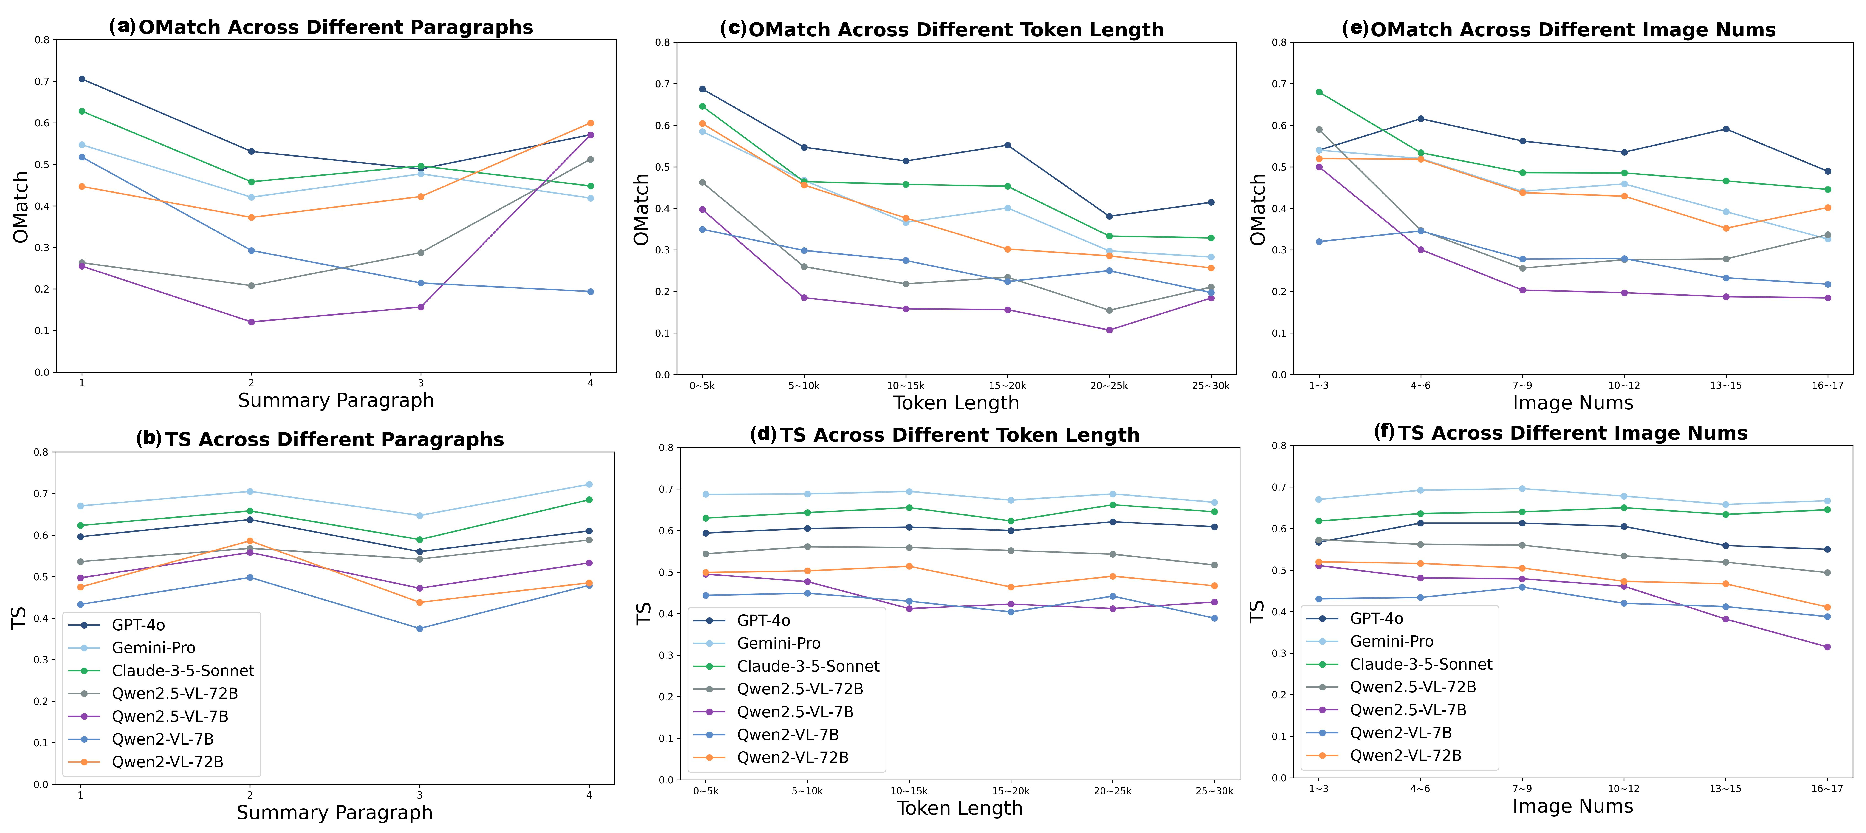
\includegraphics[width=1.0\textwidth]{figs/fig_analysis}
\caption{Quantitative analysis of the performance trends of different models as data characteristics vary, including the different paragraphs in the interleaved summarization, the token length of the original text, and the number of input images.}
\label{fig:analysis}
\end{figure*}


\subsubsection{Image Reference Bias}
\begin{table}[tbp]
\caption{All image reference results are ``None".}

\centering
\resizebox{0.45\textwidth}{!}{
\begin{tabular}{lccccc}
\toprule
& ImgAcc & NonAcc & OMatch & JacSim & IS  \\
\midrule
``None" &  0 & 1.000 & 0.325 & 0 & 0 \\
\bottomrule

\end{tabular}
}
\label{tab:bias}
\end{table}
Notably, as shown in Table~\ref{tab:bias}, when assuming all output referenced images are ``None", the OMatch score is 0.325, indicating that only 32.5\% of paragraphs actually do not require images. Considering all image metrics together, when both ImgAcc and JacSim are closer to 0 and NonAcc is closer to 1, it indicates that the model has a greater tendency not to select images. This extreme phenomenon explains the lower image-related scores for LVLMs such as InternVL-2 and InternVL-2.5.

\begin{figure}[t]
\centering
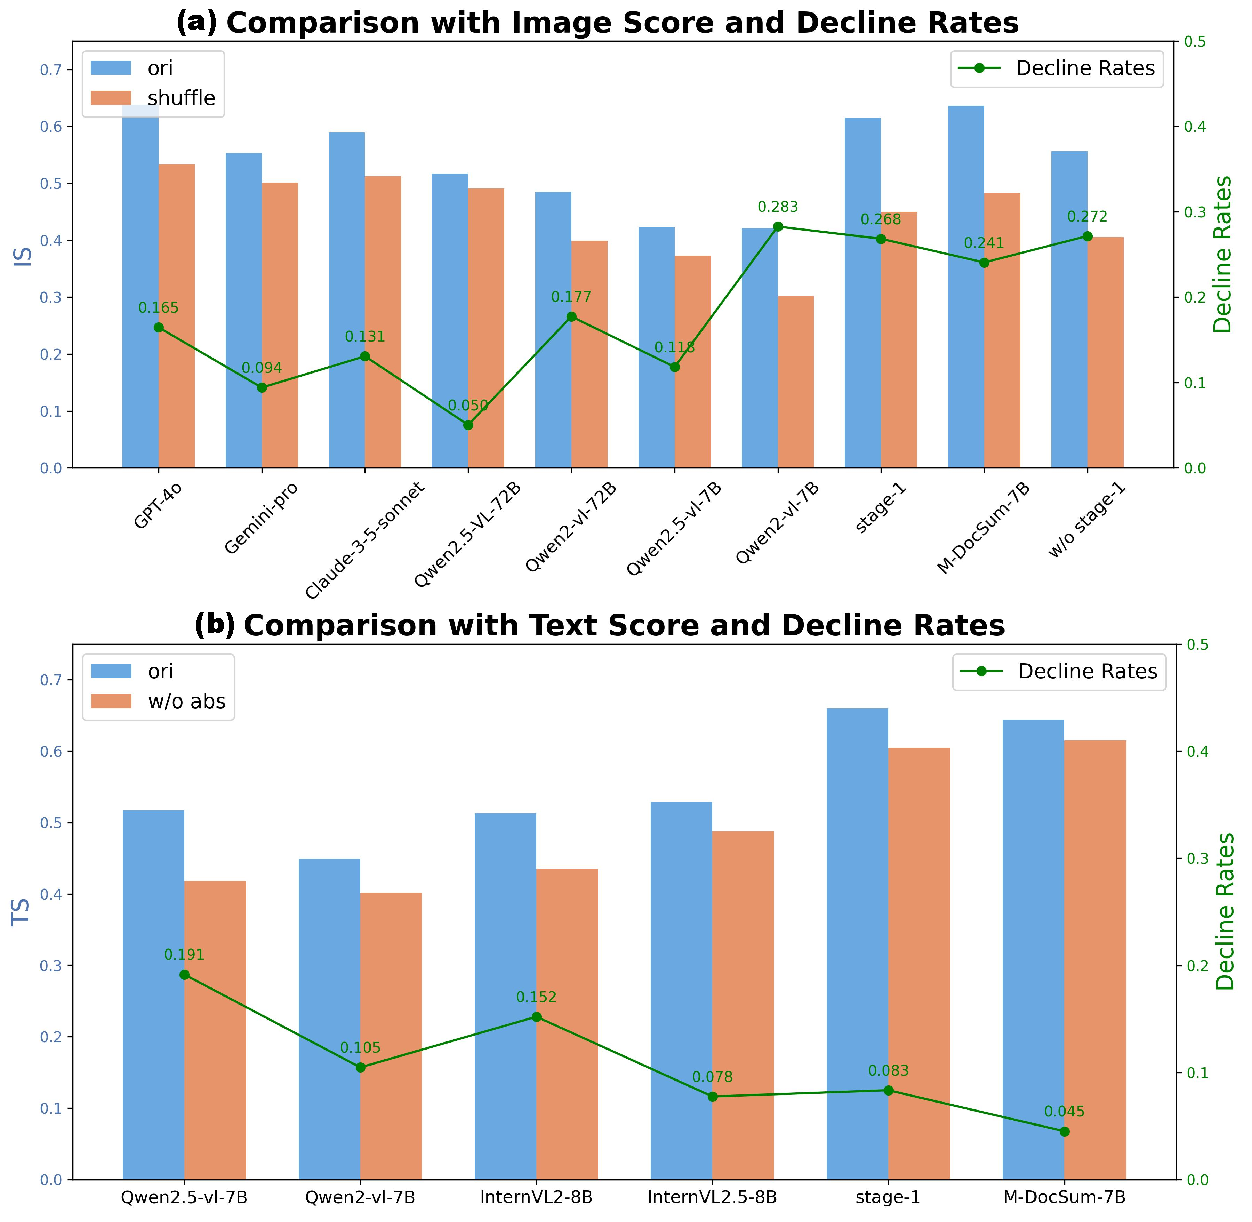
\includegraphics[width=0.49\textwidth]{figs/ablation}
\caption{Blue bars represent original image scores, orange bars represent scores after modification, and the green line indicates the decline rate.}
\label{fig:ablation}
\end{figure}


\subsection{Ablation Study}
In our ablation study, we test the robustness of LVLMs by shuffling the order of images and removing the original abstract, observing the performance under this out-of-distribution (OOD) condition.
A fundamental hypothesis is that models should primarily rely on the semantic association between images and text rather than the positional arrangement of images. 
If a model accurately captures these semantic relationships, its performance should remain stable even when the image order is changed; conversely, it indicates the model may merely have learned specific patterns.
As shown in Figure~\ref{fig:ablation}(a), overall, closed-source models or larger models exhibit lower sensitivity to image position, with performance decline rates all below 17.7\%. 
In contrast, smaller open-source models, such as Qwen2-VL-7B, demonstrate the poorest robustness. After the first stage of training, while overall performance improves, decline rates are reduced, indicating an enhanced understanding of interleaved image-text information, but not eliminating the dependence on image order. 
With the second stage of training, M-DocSum-7B exhibits even greater robustness. 
Furthermore, experimental results demonstrate that effective first-stage training is essential, if second-stage training is conducted directly, the model's decline rates actually increase.

Another question is whether the model completes the summarization by directly copying the original abstract. 
To investigate this, we conduct experiments on models of the same size with strong textual capabilities.
As shown in Figure~\ref{fig:ablation}(b), the results show that as we progressively train the model, the text score gradually increases while the decline rates decrease.
This effectively demonstrates the effectiveness of the training and indicates the continuous improvement of the robustness.
Furthermore, compared to the disturbance caused by image changes, the absence of the abstract has a weaker impact on the summarization ability, which indirectly confirms the model's low dependence on the original abstract.
Detailed results can be found in the Appendix Section~\ref{Ablation}.




\subsection{Case Study}
We provide two detailed case studies in the Appendix, Figure~\ref{fig:case_en_2} and~\ref{fig:case_en_1}.
Notably, the order of images presented in the case studies may differ from the order in the abstract. 
This discrepancy underscores a common challenge in current vision-language tasks: models often struggle to accurately capture fine-grained correspondences between images and text. 
Furthermore, the case studies clearly illustrate that existing models are prone to confusion when dealing with images that are semantically similar but possess distinct visual details, leading to inaccurate reasoning results. 